\chapter{Implementation}

This chapter focuses on the actual implementation of the algorithm and the \textit{implementation-level} optimizations, which --- along with the \textit{algorithm-level} optimizations presented in the previous chapter --- allow for the real-time execution of the algorithm.

First a short introduction to the utilized SSE instruction set extension is given, followed by the techniques employed in the acceleration of the error stack calculation, which include a rearrangement of the snapshot memory along with a separation of the required bilinear interpolation. The next section focuses on the minimum error search and the index space refinement, where a coordinate transformation is applied in order to reduce the required bit depth and to simplify the calculation of the quadratic approximations. The last section describes a fast version of the local environment map for which the Gaussian probability distributions are precalculated for a discrete parameter set.

\section{Short introduction to SSE}

SSE (Streaming SIMD Extensions) is one of the families of SIMD instruction set extensions available on x86- and x64-processors. The original SSE instructions were expanded by incremental updates, namely SSE\,2, SSE\,3, SSSE\,3, SSE\,4.1 and SSE\,4.2. The target platform supports all extensions up to SSSE 3. This implementation will mostly make use of the integer instructions provided by SSE 2 and SSSE 3.

SSE adds sixteen (eight on 32-bit platforms) new 128-bit registers to the processor, which may either hold two double- or four single-precision floats or $4 \times 32$-bit, $8 \times 16$-bit or $16 \times 8$-bit integers, thus allowing up to $16 \times$ parallel execution on a single processor core. The data layout solely depends on the instructions used on these registers. A 128-bit data block is hereinafter referred to as \textit{SSE word}.

The SSE instructions can be accessed in high level programming languages using so called \textit{intrinsics}, which behave like normal functions operating on a 128-bit data type (\texttt{\_\_mm128i} for integers, \texttt{\_\_mm128d} for doubles and \texttt{\_\_mm128} for singles) but receive special handling from the compiler and are (most of the time) translated into a single SSE instruction.

See the \textit{Intel 64 and IA-32 Architectures Optimization Reference Manual} \citep{IntelOptimizationHandbook} for more information on this topic.

\section{Error stack calculation}

\label{sec:error_stack_sse}

This section focuses on the optimizations that allow a very fast calculation of the error stack layers $\img{E}_i$. These optimizations include a special snapshot memory layout suitable for SSE as well as exploiting the separability of the motion field equation.

\subsection{Snapshot memory layout}

\begin{figure}[tb]
 \begin{center}
  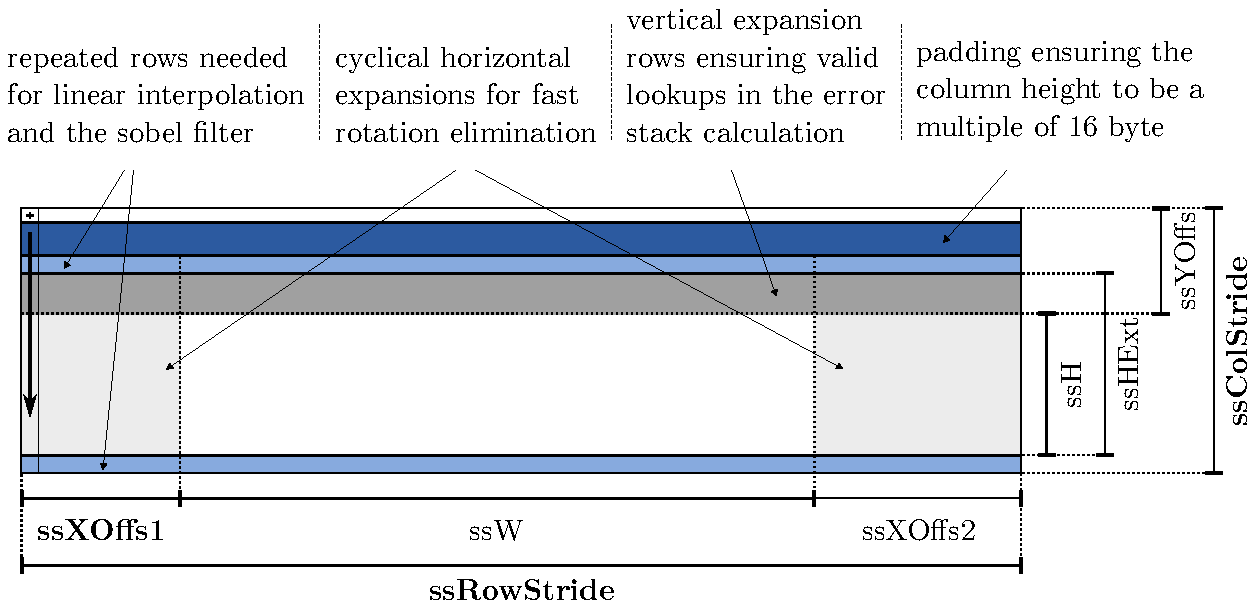
\includegraphics[width=0.975\textwidth]{media/memlayout_snapshot2.pdf}
 \end{center}
 \caption{Snapshot memory layout. Each resolution level and each snapshot component is stored according to the scheme shown above. The cross in the top left corner marks the origin, the arrow indicates the column-major memory layout. Bold labels represent values which are chosen as multiples of sixteen. The actual data used for the error stack calculation is stored in the white area in the middle of the image.}
 \label{fig:memlayout_snapshot2}
\end{figure}

\label{sec:memory_layout}

Incoming panoramic snapshot images are rearranged in memory according to a special memory layout scheme which meets the demands of the SSE implementation. This rearrangement is employed after the resolution pyramid has been calculated (see section \ref{sec:coarse_to_fine_implementation}). Once the first stage of the rearrangement has been performed (except for the transpose and horizontal expansion step, see below) the first derivatives in $x$- and $y$-direction are approximated using a $3\times3$-Sobel filter. The resulting image components (intensity, $x$-derivative, $y$-derivative) are stored individually as independent images. This corresponds to the so called \textit{structure of arrays} (SoA) paradigm, which in conjunction with SSE performs better for most applications than the classical \textit{array of structures} (AoS) \citep[chapter 4.5.1, ``data structure layout'']{IntelOptimizationHandbook}.

\paragraph{Column-major layout:} The first design decision regarding rearrangement includes a conversion from the standard row-major to a column-major memory format (hence the image is stored transposed). A column-wise processing enables the efficient interpolation scheme presented below (see section \ref{sec:motion_field_separability}). In order to save memory (and thus expensive memory access), the bit depth of the input images remains unchanged and each pixel is stored as an 8-bit unsigned integer.

By adding padding-rows, it is ensured that the column height is a multiple of 16 bytes. This is important, as SSE load instructions work most efficiently if the memory addresses are aligned to 16-byte boundaries \citep[chapter 4.4, ``stack and data alignment'']{IntelOptimizationHandbook}. Additionally, this allows each column to be handled with an integral count of SSE words.

\paragraph{Horizontal rotation elimination borders:} In order to facilitate the rotational motion elimination described in equation \ref{eqn:rot_motion_elim}, the snapshot image is cyclically extended in $x$-direction. As the panoramic images are cyclic in horizontal direction this allows the rotational motion elimination to be reduced to two horizontal offsets for the current view and the snapshot images.

However, the maximum rotational angle that can be eliminated is now limited by the width of the cyclic extension, which is currently chosen as $\frac{w}4$ in both directions, limiting the maximum rotation angle to $\pm 90^\circ$ (which should be sufficient). It should also be noted that the use of discrete pixel offsets introduces a quantization error with respect to the rotation angle, which is especially large for lower resolution levels.

\paragraph{Vertical lookup extension:} As noted in section \ref{sec:panoramic_image}, only a portion of the polar range available in the snapshot is effectively used for the actual depth reconstruction. The preprocessing step only copies this reduced portion, yet as warping the snapshot requires lookups which lie outside this reduced polar range (see figure \ref{fig:flow_template_regions}), some additional vertical extension rows allowing these lookups are added to the top of the snapshot. The height of this extension region is chosen to be as large as possible (only rows that are present in the input image are copied) and as small as needed (only rows that are referenced by the longest flow vector are copied).

If the polar range covered by the input image is too small, the vertical lookup region does not eliminate the need of adding some mechanism to the error stack calculation that allows to cope with such invalid lookups.

A copy of the top row is added to the top of the snapshot data and the same procedure is analogously performed at the bottom. This allows to prevent branching in the border regions for the linear interpolation and the Sobel–kernel application.

\paragraph{Memory layout descriptors:}

A schematic showing the complete memory layout can be seen in figure \ref{fig:memlayout_snapshot2}. The annotated widths and heights fully describe the memory layout and together form a \textit{memory layout descriptor}. These descriptors (also including the flow template and error stack memory layout data not described here) are calculated once for each pyramid level. A pointer to the memory descriptor is then passed to all parts of the implementation.

\subsection{Separability of the motion field equation}

\begin{figure}[tb]
 \begin{center}
  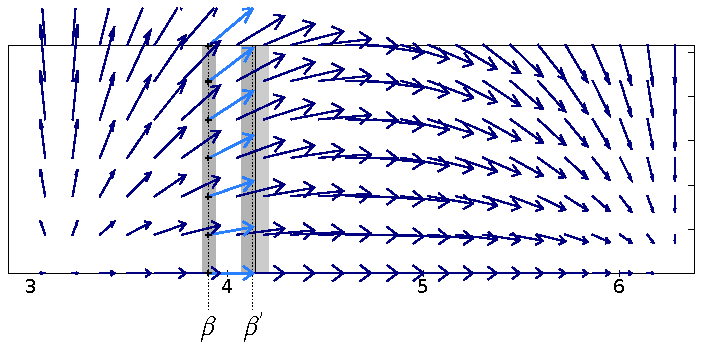
\includegraphics[width=0.75\textwidth]{media/flow_template_lookup.pdf}
 \end{center}
 \caption{Section of a flow template $\img{U}_i$. The highlighted arrows point from a target column $\beta$ (corresponding to a discrete pixel) to the source column $\beta'$. As all arrows point to the same source row, the bilinear interpolation employed when calculating the warped image $\img{SS'}_i$ can be split into a \textit{horizontal} interpolation step (interpolating between the two referenced source rows) and a \textit{vertical} interpolation step.}
 \label{fig:flow_template_lookup}
\end{figure}

\label{sec:motion_field_separability}

The motion field equation \ref{eqn:flow_template} as given in section  \ref{sec:flow_template_calculation} describes the mapping of a target pixel $(\beta, \gamma)$ in $\img{SS'}_i$ (needed for the error stack calculation, see section \ref{sec:error_stack}) to a source pixel $(\beta', \gamma')$ in $\img{SS}$. Thus the $\img{SS'}_i$ are calculated by warping the snapshot image $\img{SS}$ according to the flow template $\img{U}_i$ using bilinear interpolation. As noted above, the source column $\beta'$ solely depends on the target column $\beta$ and not on the target row $\gamma$.

Column-wise calculation of each discrete target column $\beta$ allows for separation of the bilinear interpolation into a \textit{horizontal} and a \textit{vertical} interpolation step. For the horizontal interpolation, the two neighboring source columns referenced by $\beta'$ are interpolated, resulting in an intermediate source column. In the vertical interpolation step for each row $\gamma$ in $\beta$ the two source pixels referenced by $\gamma'$ in the intermediate source column are interpolated (see figure \ref{fig:flow_template_lookup}).

\subsection{Flow template calculation}

The actual flow template data for all $\img{U}_i$ and all resolution levels are precomputed for each pixel as defined in equation \ref{eqn:flow_template_definition}. In order to simplify the code the depression angle $\check \gamma$ is set to a fixed value of $0^\circ$, while the elevation angle $\hat \gamma$ remains a free parameter.

Instead of storing a field of two-dimensional floating point vectors for each target pixel, the flow template is encoded in memory using a set of five integer arrays:
\begin{itemize}
 \item A one-dimensional 16-bit array \texttt{tarX} (size $w$) holds the index of the left-most of the two discrete source columns corresponding to each target column $\beta$.
 \item A one-dimensional array \texttt{facX} (size $w$) holds the horizontal interpolation factors for the two source columns. The factors are multiplied by $2^6$ and stored as $2 \times 8$-bit tuples. The full 8-bit range is not used in order to prevent overflows in subsequent steps.
 \item A two-dimensional 8-bit array \texttt{offsY} (size $w \times \frac{h}8$) holds the index of the first source pixel (clamped to zero) in the intermediate column for each block of eight pixels in each target column.
 \item For each pixel the two-dimensional 8-bit array \texttt{shuffleMaskY} (size $w \times 2 \cdot h$) holds the two vertical source pixel indices relative to the first source pixel offset stored in \texttt{offsY}. Inaccessible pixels --- those with an index smaller than zero or larger than fifteen --- are marked with 0xFF.
 \item A two-dimensional array \texttt{facY} (size $w \times h$) holds the vertical interpolation factors for the two source pixels corresponding to each target pixel. The values are encoded as described for \texttt{facX}.
\end{itemize}
The two-dimensional arrays are stored column-major and with corresponding padding ensuring the column size to be a multiple of 16. The offsets stored in \texttt{tarX} and \texttt{offsY} directly address the pixels as they are stored in the snapshot memory layout.

\subsection{Snapshot warping and error stack calculation}

\begin{figure}
 \begin{center}
  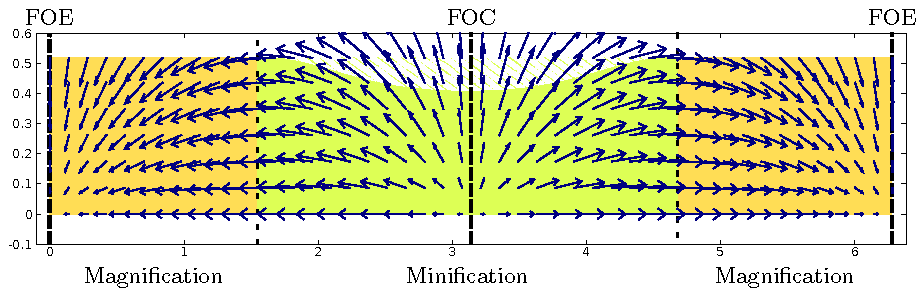
\includegraphics[width=0.975\textwidth]{media/flow_template_regions.pdf}
 \end{center}
 \caption{Regions in each flow template. The $\pi$-interval surrounding the focus of contraction (FOC) describes a \textit{minification} in which the source pixel region is always larger or equal in size to any region of target pixels (many pixels are mapped to few pixels). The $\pi$-interval surrounding the focus of expansion (FOE), however, describes a \textit{magnification} in which the source pixel region is always smaller or equal in size to any region of target pixels (few pixels are mapped to many pixels). The hatched region in the image contains the flow vectors pointing to invalid (out of range) source pixels.}
 \label{fig:flow_template_regions}
\end{figure}

The calculation of a single error stack layer $\img{E}_i$ consists of the following steps: For each snapshot component, a warped version of that component is calculated according to the flow template using bilinear interpolation. Then the absolute difference between the warped image component and the corresponding current view image component is calculated. This value is subsequently added to the resulting error stack layer value (remember that the optical flow as defined in equation \ref{eqn:optical_flow} uses the $L^1$-norm).

\paragraph{Image warping and interpolation:} Given the precalculated flow template, the horizontal and vertical warping and interpolation steps become equally trivial, although the vertical interpolation requires additional attention.

Of special interest in both steps is the SSSE 3 \texttt{\_mm\_maddubs\_epi16} intrinsic, which takes two $16 \times 8$-bit SSE words ($a$ and $b$) as input and calculates a $8 \times 16$-bit output vector $c$ according to the following expression ($[i]$ corresponds to the $i$th cell in the SSE word):
  $$c[i] = a[2 \cdot i] \cdot b[2 \cdot i] + a[2 \cdot i + 1] \cdot b[2 \cdot i + 1] \quad \forall \; 0 \leq i < 8 \; .$$
Interpolation between pixel pairs can be achieved by placing each pair in adjacent cells in $a$ and the corresponding interpolation factors in $b$, allowing eight result pixels to be computed in a single instruction.

The interpolation in horizontal direction is performed by interlacing two $16 \times 8$-bit SSE words read from the source rows into two pixel pair vectors $aLO$ and $aHI$ and interpolating those according to the factors stored in the flow template \texttt{facX} array. The two result vectors are then packed into the 8-bit intermediate column (see appendix \ref{code:horz_interpolation} for the complete code).

Interpolation in vertical direction is done by reading a $16 \times 8$-bit SSE word from the intermediate row starting with the pixel specified in \texttt{offsY} and building a single pixel pair vector by shuffling this 16-pixel input word according to the indices specified in \texttt{shuffleMaskY}. The pixel pairs are then interpolated according to the interpolation factors in \texttt{facY}. Note that this technique is only capable of mapping a maximum of 16 consecutive source pixels to 8 target pixels, so the minification factor should never exceed two (see figure \ref{fig:flow_template_regions}). Yet for the parameters used in practice this is never the case.

For invalid pixel lookups --- those marked with 0xFF in the shuffle mask --- a ``maximum error mask'' is created from the shuffle mask and the corresponding error values are set to this maximum error value. As three image components are processed and the maximum pixel intensity difference is 255 per component, this maximum error value is chosen as 0x3FF (see \ref{code:vert_interpolation} for the complete code).

\paragraph{Error stack bias:} The error bias $\tau \cdot i$ introduced for the minimum error search in section \ref{sec:minimum_error_search} is directly added to the error values in each error stack layer $\img{E}_i$ and will thus not be regarded in the following sections.

\section{Index field calculation}

The next step in the algorithm is to find the minimum error in the error stack layers and to generate the index field $\img{J}$, which is then refined to the index field $\img{\tilde J}$. Yet before these steps can be discussed in detail, an error propagation matrix $W_{\vec p}$ (left open in section \ref{sec:minimum_error_search}) needs to be chosen.

\subsection{Propagation matrix and minimum error search}

\label{sec:propagation_matrix_choice}

The most influential parameter from an efficiency point of view is the propagation matrix $W_{\vec p}$. The space and data variant $n \times n$ error propagation matrix (where $n = 2 \cdot r_W + 1$) introduced in section \ref{sec:convolution_kernels} is generally non-separable and thus needs $n^2$ calculations in every pixel. Additionally, creating and storing the filter kernels requires additional time and storage.

Preceding experiments (see section \ref{sec:results_propagation} for the results and chapter \ref{sec:experiments} for the test set-up) have shown that choosing $W_{\vec p}$ as a space-invariant $3 \times 3$ binomial convolution kernel provides an acceptable trade-off between speed and quality. The propagation matrix $W$ is subsequently defined as:
  $$W := W_{\vec p} = \frac{1}{16} \cdot \begmat 1 & 2 & 1 \\ 2 & 4 & 2 \\ 1 & 2 & 1 \finmat \; .$$
The filter is separable into a horizontal and vertical convolution
  $$W := \frac{1}{16} \cdot \begmat 1 & 2 & 1 \finmat \ast \begmat 1 \\ 2 \\ 1 \finmat$$
which can both be trivially implemented using SSE.

\paragraph{Minimum error search:} The minimum error search leading to the index field $\img{J}(\vec p)$ is implemented exactly as defined in equation \ref{eqn:kernel_minimum_search_bias}: First $\img{E}_i \ast W$ is calculated for all error stack layers (which as noted above already contain the bias $\tau \cdot i$), then for each pixel $\vec p$ the layer index with minimum error is searched. Using SSE, eight pixels can be processed at a time. In order to allow for a refinement of the index field, the indices are stored as 16-bit fixed point numbers with the scale factor $2^8$.

\subsection{Index field refinement}

In equation \ref{eqn:index_field_refinement} the refined index field $\img{\tilde J}$ was effectively defined as
\begin{equation}
\img{\tilde J}(\vec p) = \argmin_{\img{J}(\vec p) - 1 \leq j \leq \img{J}(\vec p) + 1}
  \left( \check E_{\vec p}(j) + \check R_{\vec p}(j) \right) \; ,
  \label{eqn:index_field_refinement_impl}
\end{equation}
where $\check E(J)$ refers to the convoluted quadratic error stack approximation functions and $\check R(j)$ to the convoluted regularization functions:
\begin{align*}
   \check E_{\vec p}(j) &= \sum_{\vec q \in A(\vec p)} \omega_{\vec p}^{\vec q} \cdot \tilde E_{\img{J}(\vec p)}(j; \vec q) \; ,
 & \check R_{\vec p}(j) &= \lambda \cdot \sum_{\vec q \in A(\vec p)} \omega_{\vec p}^{\vec q} \cdot (\img{J}(\vec q) - j)^2 \; .
\end{align*}


\paragraph{Simplification of the index field refinement equation:} The convolution over a set of quadratic polynomials is impractical for a fast implementation. It would be of advantage if the convoluted error stack layers $\img{E}_i \ast W$ calculated in the previous step could be reused.

In the case of $\check E_{\vec p}(j)$, the convolution and the calculation of the quadratic coefficients are commutative: For $i \in \{-1, 0, 1\}$ and $j = \img{J}(\vec p)$ the following relation holds
\begin{equation*}
  \check E_{\vec p}(j + i)
  {\overset{\text{Def. }\tilde E\vphantom{\omega_{\vec p}^{\vec q}}}=} \sum_{\vec q \in A(\vec p)} \omega_{\vec p}^{\vec q} \cdot \img{E}_{\img{J}(\vec p) + i}(\vec q) \\
  \overset{\text{Def. }\omega_{\vec p}^{\vec q}}= \left(\img{E}_{\img{J}(\vec p) + i} \ast W\right)_{\vec p}
\end{equation*}
and --- as each quadratic polynomial is uniquely defined by three points --- proves that fitting the coefficients according to the values in the convoluted error stack layers is equivalent to convolving the polynomials themselves.

Unfortunately the regularization function $\check R_{\vec p}(j)$ is not commutative regarding the convolution of the index field $\img{J}$. Expanding $\check R_{\vec p}(j)$ yields
\begin{align*}
  \check R_{\vec p}(j) &= \lambda \cdot \left(
    j^2 - 2 \cdot (\img{J} \ast W)_{\vec p} \cdot j +
    \smash{\sum_{\vec q \in A(\vec p)}} \omega_{\vec p}^{\vec q} \cdot \img{J(\vec q)}^2 \right)\vphantom{\sum_{\vec q \in A(\vec p)}}
\end{align*}
where the constant term plays no role for finding the minimal $j$. Thus an equivalent and commutative regularization function is given by
\begin{equation}
  \tilde R'(j; \vec p) = \lambda \cdot ( j^2 - 2 \cdot \left(\img{J} \ast W \right)_{\vec p} \cdot j)
\end{equation}

\paragraph{Quadratic approximation calculation:}

\begin{figure}[t]
  \begin{center}
   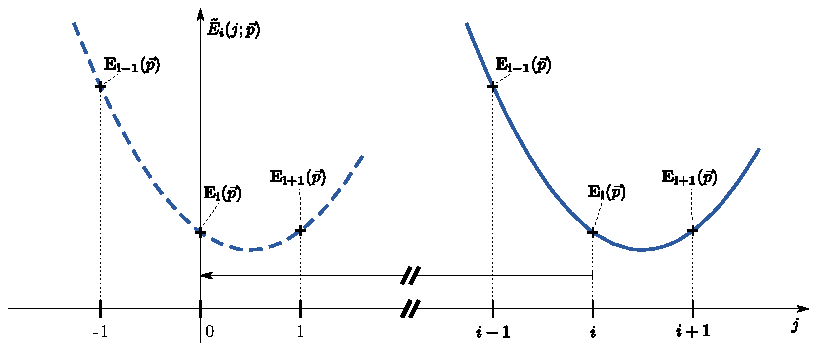
\includegraphics[width=0.975\textwidth]{media/polynomial_coord_trafo.pdf}
  \end{center}
  \caption{Translating the center index $i$ of each quadratic approximation polynomial $\tilde E_i(j; \vec p)$ (solid blue line) to the origin at $0$ (dashed blue line) allows for simplified  calculation of the polynomial coefficients $\vec w$ and lowers the required bit depth needed to store those.}
  \label{fig:polynomial_coord_trafo}
\end{figure}


The calculation of the quadratic polynomials $\tilde E_i(j; \vec p) = (j^2, j, 1) \cdot \vec w$ as given in equation \ref{eqn:polynomial_coeffs} can be simplified by a coordinate transformation which translates the center index $i$ to the origin at $j = 0$ (see figure \ref{fig:polynomial_coord_trafo}). The adapted refinement equation \ref{eqn:index_field_refinement_impl} is then given as
\begin{equation}
\img{\tilde J}(\vec p) =\argmin_{- 1 \leq j \leq 1} \left(
  \check E_{\vec p}(j) + \check R_{\vec p}(j)\right) + \img{J}(\vec p) \; .
\end{equation}
The coefficients $\vec w$ of $\check E_{\vec p}(j)$ can now be trivially implemented in SSE:
\begin{equation}
	\vec w = \begmat w_2 \\ w_1 \\ w_0 \finmat = \frac{1}2
	\begmat
		1 & -2 & 1 \\
		-1 & 0 & 1 \\
		0 & 2 & 0
	\finmat
	\cdot
	\begmat
		\mathbf{E}_{i - 1}(\vec p) \ast W \\
		\mathbf{E}_{i}(\vec p) \ast W \\
		\mathbf{E}_{i + 1}(\vec p) \ast W
	\finmat
	\label{eqn:polynomial_coeffs_impl} \; .
\end{equation}
Additionally, this equation has the advantage of yielding a much smaller coefficient vector, which can (using the SoA paradigm) be stored in three $8 \times 16$-bit SSE words \texttt{w0}, \texttt{w1}, \texttt{w2}, allowing the refinement of eight pixels at the same time.

For the regularization term $\tilde R'(j; \vec p)$ the coordinate transformation yields the following equation
$$\tilde R'(j; \vec p) = \lambda \cdot (j^2 - 2 \cdot (\left(\img{J} \ast W\right)_{\vec p} - \img{J}(\vec p)) \cdot j) \; .$$
Note that for the search range $-1 \leq j \leq 1$ the quadratic term $j^2$ is negligible and the factor two can be condensed into $\lambda$. Thus the regularization is reduced to subtracting $\lambda \cdot (\left(\img{J} \ast W\right)_{\vec p} - \img{J}(\vec p))$ from the linear coefficient vector \texttt{w1}.

All coefficients are stored as fixed point numbers (scale factor $2^3$) allowing a slightly higher resolution for $\lambda$.

\paragraph{Refined index calculation:} The extremum of a quadratic polynomial $w_2 j^2 + w_1 j + w_0$ is given by $\check \jmath = - \frac{w_1}{2 w_2}$. In order to eliminate the need for special handling (which is hardly possible when using SIMD instructions) in the case of $w_2 = 0$, $w_2$ is always set to one in that case. The resulting $\check \jmath$ is clamped to the interval $[-1, 1]$ and the corresponding error value is then compared to the error values at $j = -1$ and $j = 1$. The actual refined index field entry is then chosen as the index belonging to the smallest of the three error values.

As SSE does not provide integer division instructions, the term $-\frac{w_1}{2 w_2}$ is evaluated using floating point numbers. The approximative but significantly faster reciprocal instruction $\texttt{\_mm\_rcp\_ps}$ in conjunction with a multiplication is used here, which has a combined precision in the range of $\approx 2^{-11}$ \citep[chapter 11.12 ``divide and square root operations'', p. 417ff.]{IntelOptimizationHandbook}. This is not a problem since the resolution of the fixed-point 16-bit indices $j$ was chosen as $2^{-8}$.


\section{Local environment map}

The local environment map is especially optimized in the position update and the distribution accumulation as introduced in section \ref{sec:obstacle_detection}. These optimizations are roughly sketched in the two following sections.

\subsection{General optimizations}

The local environment map is stored in memory as a 16-bit two-dimensional matrix. SSE trivially allows to speed up the map decay step (equation \ref{eqn:map_decay}), as the SSSE 3 intrinsic \texttt{\_mm\_mulhrs\_epi16} allows $8\times$ parallel multiplication of a $8 \times 16$-bit word with a scalar $\delta \in (0, 1]$.

Furthermore the need of the image rotation in the map update step was eliminated by integrating the change in orientation $\psi$ and using this current orientation and the current translatory motion direction $\alpha$ as an angular offset when inserting the Gaussian distributions. This allows to reduce the map update step to a discrete, pixel wise translation. The error introduced by rounding to discrete pixel offsets is accounted for by feeding the rounding error into the next map update step (comparable to error-diffusion dithering).

Although the calculation of the thresholded map image can be parallelized using SSE, no trivial optimization of the connected component calculation was found.

\subsection{Distribution accumulation optimization}

\begin{figure}[tb]
 \begin{center}
  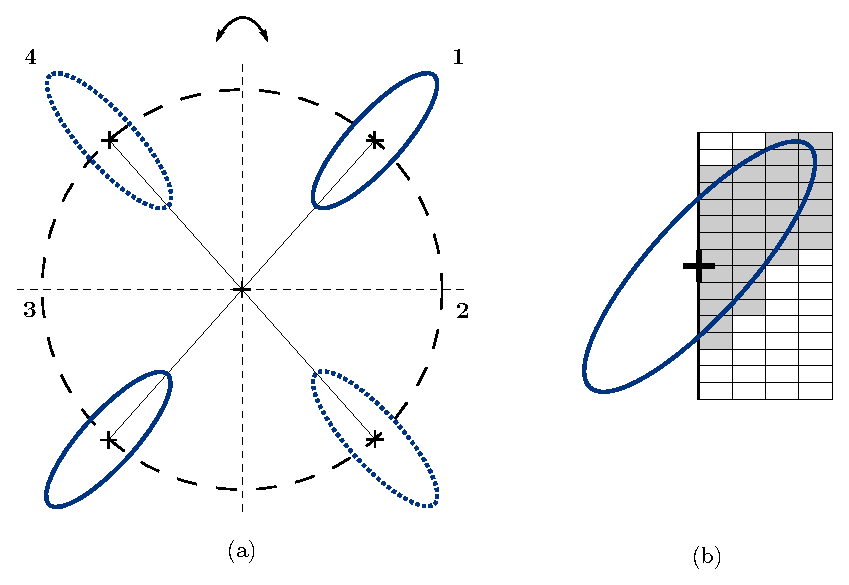
\includegraphics[width=0.975\textwidth]{media/gaussian_distribution_symmetries.pdf}
 \end{center}
 \caption{Symmetries of a Gaussian distribution. (a) A Gaussian distribution calculated for quadrant 1 can be used in quadrant 3 without modification. Mirroring along the $x$-axis allows to use the distribution in quadrant 2 and 4. Consequently precalculating the distributions for one quadrant only allows to reduce the space requirement by one quarter. (b) As each Gaussian distribution is point-symmetric, only one half of the distribution needs to be stored in memory --- the memory footprint can be reduced even more by skipping all SSE words which only contain pixel values below a certain threshold (white).}
 \label{fig:gaussian_distribution_symmetries}
\end{figure}

In order to avoid the costly evaluation of the Gaussian probability distributions whenever a landmark point $\vec q = (\beta, r)$ is inserted into the map, the distributions are precalculated in Cartesian space for discrete $\beta_i \in [0, 2\pi]$ and a discrete range of $r_i \in [r_{\mathrm{MIN}}, r_{\mathrm{MAX}}]$. Note that the variance $\sigma_r$ as derived in equation \ref{eqn:sigma_r} also depends on the translatory distance $d$ between $\img{SS}$ and $\img{CV}$, yet precalculating the distributions for a three-dimensional parameter space $\beta, r, d$ is impractical. Therefore the robot is implicitly assumed to move with constant speed.

As depicted in figure \ref{fig:gaussian_distribution_symmetries}, the distributions are stored as fixed point $8 \times 16$-bit SSE words for a rectangular hull encompassing a contour line at a certain threshold level. To lower the memory requirements symmetries in the distributions are exploited and only SSE words containing values above the threshold level are stored in memory, along with a descriptor that contains the number of words skipped and the number of words in a row. Preceding experiments have shown that the reduced memory footprint and better cache locality outweighs the overhead introduced by this packing scheme.

The map array size is extended by the half width/height of the largest Gaussian distribution bounding rectangle in order to eliminate the need of border handling (and thus branching) when plotting the map pixels.

The SSE code used for accumulating a precalculated distributions onto the local environment map is given in appendix \ref{code:gauss}.

